\documentclass[12pt]{scrartcl}
\usepackage[utf8]{inputenc}
\usepackage[ngerman]{babel}
\usepackage[pdfusetitle]{hyperref}
\usepackage{graphicx}
\usepackage{calc}
\usepackage{fancyhdr,multicol,multirow,paralist,graphicx,array,enumitem}
\usepackage{amsmath}
\usepackage{color}
\usepackage[dvipsnames]{xcolor}
\addto\captionsngerman{
  \renewcommand{\contentsname}
    {Index}
}
\KOMAoptions{parskip=half+,paper=a4,twocolumn=false,DIV=12}
\fancypagestyle{igi-style}{
\fancyhf{}
\fancyhead[L]{CI (CS) Questions}
\fancyhead[R]{IGI}
\fancyfoot[C]{\thepage}
\renewcommand{\headrulewidth}{0.4pt}
\renewcommand{\footrulewidth}{0.4pt}}
\fancypagestyle{spsc-style}{
\fancyhf{}
\fancyhead[L]{CI (CS) Questions}
\fancyhead[R]{SPSC}
\fancyfoot[C]{\thepage}
\renewcommand{\headrulewidth}{0.4pt}
\renewcommand{\footrulewidth}{0.4pt}}
\fancypagestyle{index-style}{
\fancyhf{}
\fancyhead[L]{CI (CS) Questions}
\fancyhead[R]{Index}
\fancyfoot[C]{\thepage}
\renewcommand{\headrulewidth}{0.4pt}
\renewcommand{\footrulewidth}{0.4pt}}
\setdescription{itemsep=0pt}
\makeatletter
\newenvironment{minipagespace}{
\begin{minipage}
}{
\end{minipage}
\vspace{10pt}
}
\makeatother
%\setenumerate{nosep}
\setcounter{tocdepth}{3}
\title{CI (CS) Questions}
\date{2015}
\begin{document}

\pagestyle{igi-style}

\section{IGI}

\subsection{Hypothesis for linear regression = ?}

\begin{align*}
\text{Hypothesis for one input feature: } & h_\theta(x)=\theta_0+\theta_1 \cdot x \\
\text{Hypothesis for multiple input features: } & h_\theta(x)=\theta_0+\theta_1 \cdot x_1 + \cdots + \theta_n \cdot x_n \\
\text{More compact notation: } & h_\theta(x)=x^T\theta
\end{align*}

\subsection{Cost-function for linear regression = ?}
\begin{align*}
J(\theta_0,\theta_1)= \frac{1}{m} \sum_{i=1}^{m}(h_\theta(x^{(i)})-y^{(i)})^2
\end{align*}

\subsection{How many local minima may the cost function for lin. reg. have (under regular conditions)? }
There could be multiple local minima and the algorithm (gradient descent) may get stuck in one of them, but only one global minima.

\subsection{Name two ways to minimize the cost-function}
gradient descent \\
direct analytical solution

\subsection{General gradient descent formula}
\begin{align*}
\theta_j:=\theta_j - \eta \cdot \frac{\partial}{\partial\theta_j} J(\theta_0,\theta_1)
\end{align*}

\subsection{Linear regression with gradient descent formula?}
\begin{align*}
&\theta_0:= \theta_0 - 2\eta \cdot \frac{1}{m} \sum_{i=1}^{m}(h_\theta(x^{(i)})-y^{(i)}) \\
&\theta_1:= \theta_1 - 2\eta \cdot \frac{1}{m} \sum_{i=1}^{m}(h_\theta(x^{(i)})-y^{(i)}) \cdot x^{(i)} \\
&\eta=\text{Learning Rate},x^{(i)}=\text{input},(h_\theta(x^{(i)})-y^{(i)})=\text{error} 
\end{align*}

\subsection{What issues can arise during gradient descent?}
There could be multiple local minima and the algorithm (gradient descent) may get stuck in one of them. If the learning rate is too small it leads to slow convergence, if it's too large it leads to divergence (oscillations)

\subsection{What is the design matrix? What are its dimensions?}
The design matrix is a matrix consisting of all the transposed training features, its dimensions are: $m \cdot (n+1)$ where $m$ is the number of training examples and $n$ is the number of features.

\subsection{Analytical solution for linear regression? What are its components?}
The solution can be calculated by setting all partial derivatives of the cost function to 0, then using the Moore-Penrose Pseudoinverse of the design matrix $X$ with the formula: $\theta^* = (X^T X)^{-1}X^Ty$ \\
$y$ is the output/target vector.

\subsection{Pros/Cons of gradient descent vs. analytical solution}
Gradient descent:\\
- need to choose learning rate $\eta$ \\
- iterative and needs many iterations to converge \\
+ works well even if number of input features $n$ is high \\
\\
Analytical solution: \\
+ no need to choose $\eta$ \\
+ direct solution (no iterations) \\
- slow if $n$ is too large (inverting a $n*n$ matrix)

\subsection{How can one learn non-linear hypothesis with linear regression?}
With sinusoid ($\Phi_2=cos(x)$) and quadratic ($\Phi_2=x^2$) fit, setting $\Phi_0=1, \Phi_1=x$ and $\Phi_2$ appropriately.

\subsection{What is polynomial regression?}
Features are powers of $x$, $n$ is the degree of the polynome to be learned. \\
$\Phi_0=x^0, \Phi_1=x^1, \Phi_2=x^2, \cdots , \Phi_n=x^n$

\subsection{What are radial basis functions?}
Gaussian-shaped radial basis functions: Each basis function $j$ has a center $c_j$ in the input space, and the width of the basis functions is determined by $\sigma$
\begin{figure}[htb]
  \begin{center}
  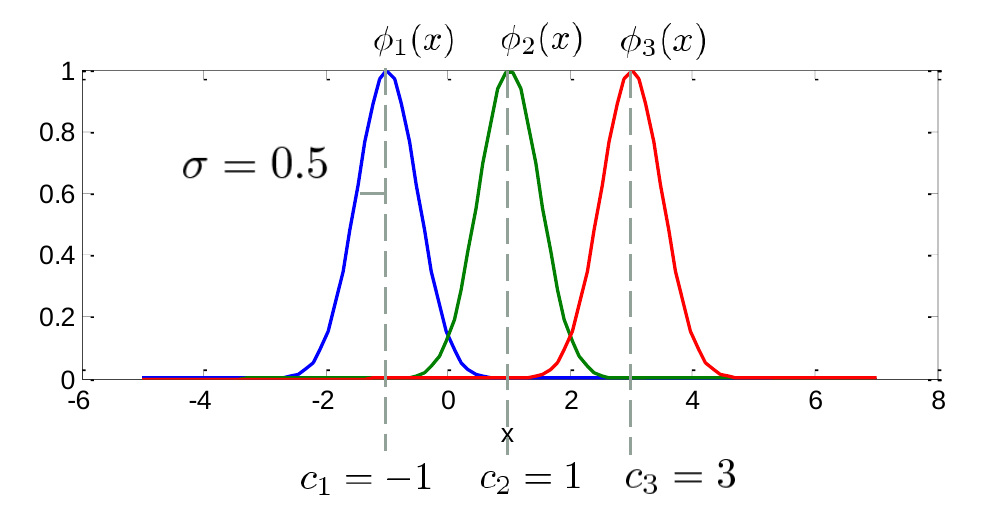
\includegraphics[scale=0.45]{gaussian-rbf}
  \end{center}
  \vspace{-\baselineskip}
\end{figure}

\subsection{Logistic regression is a method for ... regression/classification?}
{\bf The} default classification model, using binary classification with the one-vs-all algorithm.

\subsection{Logistic regression hypothesis?}
\begin{align*}
h_\theta(x) &= \sigma(x^T\theta) \\
 &= \sigma(\theta_0+\theta_1 \cdot x_1 + \cdots + \theta_n \cdot x_n)
\end{align*}

\subsection{Cost-function for logistic regression?}
How well does hypothesis fit the data? Mean over all training examples.
\begin{align*}
J(\theta_0,\theta_1) &= \frac{1}{m} \sum_{i=1}^{m}Cost(h_\theta(x^{(i)}),y^{(i)}) \\
Cost(p,y) &= -log(1-p)\text{, if }y=0 \\
 &= -log(p) \qquad \text{, if }y=1
\end{align*}

\subsection{Is the cost-function in logistic regression convex or non-convex?}
It is convex, because it gives a unique local/global minimum!

\subsection{What does ``adaptive learning rate" mean in the context of gradient descent?}
At each iteration compare the cost function value $J(\theta)$ before and after the gradient descent update. \\
If the cost increased, reject the update (go back to previous paramters) and multiply the learning rate $\eta$ by {\bf 0.7} \\
If the cost decreased proceed and multiply the learning rate $\eta$ by {\bf 1.2}

\subsection{How to evaluate a hypothesis?}
\label{traintest}By using a test set! The training set is used by the learning algorithm to find a hypothesis, the test set is an independent data set used afterwards to test the hypothesis on {\bf new (unseen) test examples}!

\subsection{What is underfitting/overfitting?}
Underfitting: Model is too {\bf simple} (often too few parameters), leads to {\bf high training error, high test error}. \\
Overfitting: Model is too {\bf complex} (often too many parameters), leads to low traning error, {\bf high test error}. \\
In between: Model has the ``right" complexity, leads to a moderate training error, {\bf lowest test error}.

\subsection{What is model selection?}
\label{model1}Used to automatically select the model complexity (hyperparameters) that is most suitable for a given learning problem. The idea is to simply try out a variety of different learning algorightms/variants and select the one with the best predictive performance.

\subsection{What are training, validation and test set?}
For training and test set see \ref{traintest} \\
\label{model2}A validation set is used to estimate the predictive performance of each learning algorithm/variant. The hypothesis with the lowest validation error is selected in model selection.

\subsection{How does model selection work (procedure)?}
See \ref{model1} \ref{model2}

\subsection{What types of neural networks are there?}
ANNs, Artificial Neural Networks (computers) and BNNs, Biological Neural Networks (the brain).

\subsection{What are ANNs?}
ANNs are computational models that model how the brain works, they are motivated and inspired by BNNs but are still only very simple imitations.

\subsection{Types of ANNs?}
\subsection{Applications of ANNs?}
Function approximation, classification, data processing, robotics, vehicle/process control, decision making (game-playing), pattern recognition.

\subsection{Artificial neuron model?}
The neurons consist of an activation function that gets a set of inputs $x_1 \cdots x_n$ that are each weighted with $w_1 \cdots w_n$. The output $z$ is produced when the neuron activates. The activation function is weighted with a bias $b$, also called threshold.

\subsection{What is an activation function, types and usage?}
Activation functions decide when to ``fire" the neuron's output.
\begin{figure}[htb]
  \begin{center}
  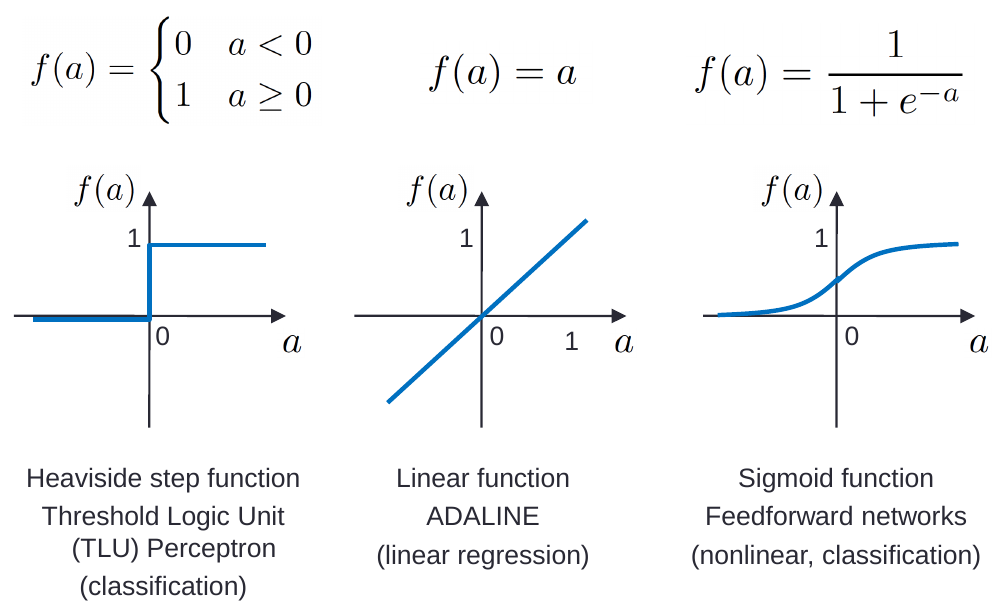
\includegraphics[scale=0.45]{activation_functions}
  \end{center}
  \vspace{-\baselineskip}
\end{figure}

\subsection{What is Perceptron?}
Perceptron is the simplest neural network for classification of linearly separable data - it is a linear (binary) classificator - consisting of one neuron with a Heaviside step function as activation function.

\subsection{Convergence properties of Perceptron?}
When the training set is linearly separable the algorithm converges.

\subsection{Binary linear classification with Perceptron?}
When the training data is linearly separable there exist parameters $w$ defining a decision boundary or a hyperplane (a subspace of one dimension less than it's ambient space) such that:
\begin{figure}[htb]
  \begin{center}
  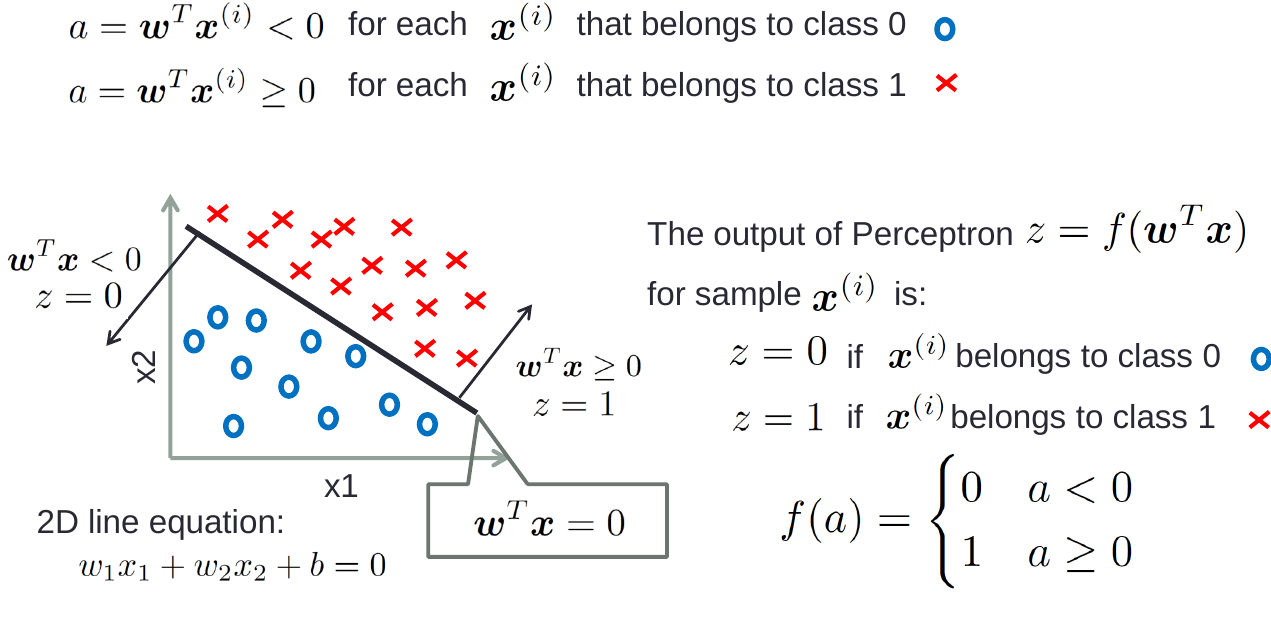
\includegraphics[scale=0.35]{perceptron}
  \end{center}
  \vspace{-\baselineskip}
\end{figure}

\subsection{Perceptron learning algorithm?}
For each sample from the training set, check if it is classified correctly, if yes then no change is made, if no then the weights are adjusted. Repeat until everything is correctly classified, the max number of iterations is reached or some other criteria (max number of misclassified samples).

\subsection{Limits of Perceptron?}
If the data is not linearly separable Perceptron cannot solve it and does not even converge. Perceptron can not solve the XOR-Problem.

\subsection{Can you use Perceptron to classify nonlinear data?}
Normally not, but with Kernel Perceptron you can separate nonlinear data!

\subsection{What is feedforward architecture?}
A network with a feedforward architecture has no cycles. The input information is propagated from the input neurons on the left (over the hidden layers in the middle) to the output neurons on the right.

\subsection{What is the hidden layer and what is it useful for?}
Hidden neurons are situated in hidden layers between input and output layers. They make it possible for a network to learn non-linear functions because they can be used to represent combinations of input features. With too many hidden neurons, the network will just memorize the input patterns ({\bf overfitting!}) and with too few hidden neurons, the network may not be able to make all the necessary generalizations ({\bf underfitting!})

\subsection{What function implements ANN with 1 hidden layer with sigmoid activation function?}
Every bounded continous function.

\subsection{Can Perceptron solve XOR? What about Multilayer Perceptron?}
No, Perceptron cannot solve XOR, but it's possible with hidden layers!

\subsection{What is the Credit Assignment Problem? In context of ANN?}
The problem deals with determining how the success of a system's overall performance is affected by it's individual components. In ANN: assign a ``blame" to each hidden neuron for it's contribution to an error on the output neuron.

\subsection{What is the backpropagation algorithm?}
Using the idea of the Credit Assignment Problem, we calculate the activatios and outputs $z$ of all neurons going forwards, then we're calculating the errors $\delta$ and propagate them back going backwards. We use this information on the errors to update the weights of the (hidden) neurons.

\subsection{What error function minimizes backpropagation?}
\begin{align*}
\frac{\partial E^{(i)}}{\partial\omega_{kj}} &= \partial_k z_j \\
E^{(i)} &= \frac{1}{2} \sum_{k=0}^K e^2_k = \frac{1}{2} \sum_{k=0}^K (z_k - y_k)^2
\end{align*}

\subsection{Why is the backpropagation algorithm used?}
Because of good results in big networks with the good GPU power nowadays, and to assign a blame to nodes in order to prevent errors.

\subsection{Weight update rules for output and hidden neurons?}
\begin{align*}
\text{Hidden Neurons: } \delta_k &= \frac{\partial f_k(a_k)}{\partial a_k} \sum_{r\in post(k)} \delta_r \omega_{rk} \\
\text{Output Neurons: } \delta_k &= \frac{\partial f_k(a_k)}{\partial a_k} e_k
\end{align*}

\subsection{What are online and batch learning? What is the difference?}
In batch learning, the error gradient for each sample from the training set is calculated and accumulated. The weight update is only done after all samples have been seen. \\
In online learning, we use the calculated error gradient for a weight update after each sample from the training set has been presented. \\
Online learning is often much faster, it can be used when there is no fixed training set (new data keeps coming), the noise in the gradient of the weight update can help to escape from a {\bf local minimum}

\subsection{How can one use ANNs for classification? And how for regression?}
For classification, we can use a sigmoid activation function in the output layer which ensures values between 0 and 1, which can help us distinguish between classes. \\
For regression, we can use a linear activation function in the output layer to provide an arbitrary output range.

\subsection{ANN properties?}
Neurobiological analogy, adaptive model, learns input output mapping, learning is slow but testing is fast, data does not have to be precise and perfect, result is not dependant on a single point of failure, very fault tolerant and robust, knowledge is stored implicitly (it is hard to interpret it)

\subsection{What is the margin of separation?}
The margin of separation is the region between classes without samples. The SVM tries to find an optimal decision boundary (hyperplane) determined by $\omega_0$ and $b_0$. For separation of two classes the separation margin must be maximized.

\subsection{What are support vectors?}
SVs are the closest points (samples) to the separation hyperplane, and they are used for defining the optimal separation hyperplane. SVs are samples for which $w_0^T x^{(i)} + b_0 = \pm 1$ holds.

\subsection{What is a SVM?}
A Support Vector Machine finds the maximum margin hyperplane, the hyperplane that maximizes the distance from the hyperplane to the closest training point(s).

\subsection{What is the separation hyperplane and the discrimination function?}
The separation hyperplane is given by $w_0^T x^{(i)} + b_0 = 0$, where the discrimation function is given by $h(x) = w_0^T x^{(i)} + b_0$. The class of a new sample is determined based on the negative or positive value returned by $h(x)$.

\subsection{What is the distance of a sample from the hyperplane?}
The distance is $r = \frac{h(x)}{||\omega_0||}$, where $||\omega_0||$ is just the euclidian norm.

\subsection{How is the margin of separation maximized?}
Maximizing the maring is equivalent to minimizing $||\omega||$, since this norm involves a square root we'd rather look at the minimization of $\frac{1}{2}||\omega_0||^2$, which does not change the solution but is easier to handle.

\subsection{Why do we use soft margin?}
For separation of classes with outliers that are not linearly separable.

\subsection{What is a kernel?}
Kernels are functions that return the inner products between the images of data points in some space. They are often interpreted as similarity measures. $K(x_1,x_2)=\varphi(x_1)^T \varphi(x_2)$ \\
\label{kernel-trick}Kernels make it possible to operate in a high-dimensional {\it implicit} feature space without ever having to compute the coordinates of the data in that space - no need for explicit mapping!

\subsection{State Cover's theorem}
Given a set of training data that is not linearly separable, one can with high probability transform it into a training set that is linearly separable by projecting it into a higher dimensional space via some non-linear transformation.

\subsection{What is the kernel trick?}
See \ref{kernel-trick} \\
This is often computationally cheaper than the explicit computation and is thus called the kernel trick.

\subsection{Conditions for the kernel matrix?}
Given by {\bf Mercer's theorem}: the kernel matrix must be symmetric positive definite. It can be calculated through the inner product between all pairs of data samples.

\subsection{Name a few standard kernels}
Polynomial kernel $K(x,y)=(x^Ty+c)^d$ \\
RBF kernel $K(x,y) = exp(-\frac{||x-y||^2}{2\sigma^2})$ \\
Sigmoid kernel $K(x,y) = tanh(ax^Ty +b)$ \\
String kernels, Graph kernels

\subsection{Multiclass vs multilabel classification}
The goal is to find a function which correctly predicts the {\bf single} class to which a new sample belongs. It is different form a multilabel classification, where the goal is to assign each sample to a set of target labels (a label having multiple classes)!

\subsection{Methods for multiclass problems}
One-vs-all (OVA), One-vs-one (OVO), Error Correcting Output Codes (ECOC)

\subsection{What is OVA?}
One-vs-all creates classifiers that distinguish each class from all other classes. There is one classifier per class: $N$ classes means $N$ classifiers.

\subsection{What is OVO?}
One-vs-one creates classifiers that distinguish between each pair of classes. That means for $N$ classes there are $N(N-1)/2$ classifiers.

\subsection{What is ECOC?}
Each class is represented by a binary code of length $n$ and each bit position corresponds to the output of a classifier. During training one classifier is trained per bit position, during testing get the output of classifiers and find the closest full binary code to decide the class, for example with euclidean distance. ECOC can recover from some bit errors caused by limited or bad features.

\subsection{What is a confusion matrix and why do we use it?}
It is an important tool for visualizing and analyzing the performance of a classifier for multiple classes. It shows for each pair of classes how many of them were incorrectly assigned, it's easy to see which classes are often confused with one another and this place containing the largest error can be improved.

\subsection{Difference between lazy and eager learning?}
Eager learning \\
The system tries to generalize the training data before receiving queries (e.g. neural networks) \\
{\color{ForestGreen} the target fuction is approximated globally during training } \\
{\color{ForestGreen} deals with noise in the training data} \\
{\color{red} unable to provide good local approximations in the target function} \\
\\
Lazy learning \\
the generalization beyond the training data is delayed until a query is made to the system (e.g. k-NN) \\
{\color{ForestGreen} the target fuction is approximated locally } \\
{\color{ForestGreen} deals with changes in the problem domain} \\
{\color{red} large space requirement to store the entire training dataset} \\ 
{\color{red} slow to evaluate }

\subsection{What is instance based learning?}
Instance based learning compares new problem instances with instances seen in the training phase (stored in memory). The hypothesis is constructed on the fly and the complexity can grow with the data (worst case: a list of all training samples) but the advantage is that the model can adapt to previously unseen data.

\subsection{What is k-NN?}
k-nearest neighbors is one of the simplest of all machine learning algorithms. Uses instance based learning (lazy learning). The main idea: \\
For a new sample examine the {\bf k} closest training samples according to some metric (most common: euclidean distance) and assign the new sample to the most frequently occuring class withing those {\bf k} samples.

\subsection{How does the number of neighbors influence k-NN?}
The best choice of k depends upon the data, larger values reduce the effect of noise but make boundaries less distinct. A good value for k can be selected by various heuristic techniques.

\subsection{Training and testing procedure for k-NN?}
Training is very fast and immediately stored in feature vectors and class labels. The samples are usually preprocessed to speed up queries (perform feature extraction and dimensionality reduction). \\
Testing: k-NN can be used for Classification, here a new sample is classified by majority votes of it's k nearest neighbors, and Regression\footnote{Regression is a statistical process for estimating the relationships among variables.}, here the value is the average of the values of it's k nearest neighbors.

\subsection{When to use k-NN, what are pros/cons?}
Use when lots of data is available and data has a small number of features. \\
Pros: easy to implement, training is very fast but can learn complex decision boundaries, no information loss (all samples are kept), can be very accurate if a lot of data is available, easy to understand and intuitively interpretated. \\
Cons: Requires a lot of memory to store all samples, slow at query time, the accuracy can be severly degraded by the presence of noisy or irrelevant features, especially in higher dimensions; sensitive to the local structure of the data, the parameter {\bf k} needs to be tuned..

\subsection{What is cross-validation?}
Split the data into training and validation set and always alternate through multiple rounds, performing the analysis on the training set and validate the analysis on the validation set. The validation results are averaged over the rounds. Used in order to limit problems like overfitting, by ``testing" the data even during the training phase.

\subsection{Types of cross-validation?}
k-fold, 2-fold, leave-one-out, repeated random sub-sampling

\subsection{Difference between 2-fold and leave-one-out cross validation?}
2-fold: used when data sets are very huge, data is split in half, one of the halves used for training the other for validation and vice-versa \\
leave-one-out: used when data sets are very small, uses one sample as validation set and the rest as training sets (k-times!)

\subsection{What is the bias-variance tradeoff?}
Bias - how accurate the model is across different training sets \\
Variance - how sensitive the model is to small changes in the training set. \\
High variance leads to overfitting and high bias leads to underfitting, to achieve good performance outside of the training set a tradeoff must be made!

\subsection{What is regularization and how is it used?}
The idea is to prevent overfitting by penalizing models with extreme parameter values. Instead of minimizing the original problem $J(\theta)$ minimize $J(\theta) + \lambda ||\theta||^2$ where $||\theta||$ is $L_2$ norm (euclidian)

\subsection{What are regularization methods for NN?}
If we assume a neural network learns the same input-output function with different number of hidden layers and parameters, then we see with fewer parameters it's more prone to underfitting and with more parameters it's more prone to overfitting. To address this issue with overfitting and keep the training error low the weights of the neural network should be kept as small as possible - using regularization! \\ \\
Weight decay - is a simple $L_2$ norm regularization for neural networks, the weights of the NN will be an additional term in the Error function: \\ $E(\omega) = MSE(\omega) + \frac{\lambda}{2}||\omega||^2$ \\ \\
Early stopping - a form of regularization which provides a guidance as to how many iterations can be run before the NN begins to overfit. The weights are initialized to small values and the learning is stopped when the error on validation data increases beyond a certain threshold.

%%%%%%%%%%%%%%%%%%%%%%%%%%%%%%%%%%%%%%%%%%%%%%%%%%%%%%%%%%%%%%%%%%%%%%%%%%%%%%%%%%%%%%%%%%%%

\newpage
\pagestyle{spsc-style}

\section{SPSC}

\subsection{Explain the problem of sequence classification using HMMs!}
\label{eval}
Evaluierungsproblem (Klassifikationsproblem): Gegeben ist das Modell $\Theta_t$ und eine Beobachtungssequenz $X = x_1, \cdots ,x_N$. Gesucht ist die Likelihood (Produktionswahrscheinlichkeit) $P(X|\Theta_t)$ einer Beobachtungssequenz. Diese Likelihood kann zur Klassifikation im Bayes Klassifikator herangezogen werden, d.h. der Bayes Klassifikator kann Sequenzen $X$ unterschiedlicher Länge klassifizieren:
\begin{align*}
P(t|X) = \frac{P(X|t)P(t)}{P(X)}
\end{align*}
Für die Likelihood Funktion $P(X|t)$ kann das Hidden Markov Model verwendet werden: $P(X|t)=P(X|\Theta_t)$ wobei $\Theta_t$ das Modell für Klasse $t$ repräsentiert. Man wählt jene Klasse $t^*$ mit der größten posterior Wahrscheinlichkeit $P(t|X)$:
\begin{align*}
t^* = \text{arg }\underset{t}{max}[P(X|t)P(t)] \text{arg }\underset{t}{max}[P(X|\Theta_t)P(t)]
\end{align*}
Die Berechnung von $P(X|\Theta_t)$ erfolgt mit dem Forward/Backward Algorithmus.

\subsubsection{Why is it in principle computationally expensive to solve?}
\subsubsection{Which property is used in the forward-algorithm to allow efficient computation?}

Prinzipiell sehr aufwendig wegen einer Rekursion.
Der Forward/Backward Algorithmus nutzt die Faktorisierungseigenschaft von $P(X,Q|\Theta)$ und kann mithilfe der Rekursion die Anzahl der Rechenoperationen auf $O(2(N_s)^2N)$ reduzieren.

\subsubsection{How could it be applied to speech recognition?}

Modelling of phonems as n-grams directly leads to useful representation as Markov chains.

\subsubsection{Can the Viterbi algorithm be used for a suitable approximation? Why/Why not?}
\label{Viterbi}
Viterbi kann nicht verwendet werden, da Viterbi eine Hidden State Sequence erzeugt, die die Beobachtungssequenz am besten erklärt.

\subsubsection{Explain the property i.i.d. (``independent and identically distributed"). Would you model data with this property using a Markov Model?}

iid heißt, das die Samples $x_1, \cdots ,x_N$ statistisch unabhängig sind und von der gleichen Wahrscheinlichkeitsfunktion stammen. Yes I would model, because you can then use the log-likelihood und damit kann man Probleme bei großen N vermeiden.

\subsection{Explain the parameters of Gaussian Mixture Models! Explain the EM algorithm that estimates these parameters}

\begin{align*}
P(X|\Theta) = \sum_{m=1}^M \omega_m \text{ } \mathcal{N}(X|\mu_m, \Sigma_m) \rightarrow \text{Sum of weighted gaussians}
\end{align*}
$\omega_i \cdots$ weight of one gaussian distribution \\
$\mu_i \cdots$ mean value of gaussian \\
$\Sigma_i \cdots$ standard deviation of Gaussian \\
$M \cdots$ number of Gaussian distributions \\
$\mathcal{N} \cdots$ Gauss Function \\
\\
EM-Algorithmus
\begin{enumerate}
\item Initialisierung: $t \cdots$ Iterationszähler
\item E(xpectation)-Step: Klassenzugehörigkeit ausrechnen \\
Dazu berechnet man die Zugehörigkeitswahrscheinlichkeit $P(m|x_n,\Theta^t)$. Diese Posteriorverteilung ist faktisch gleich dem Posterior beim Bayes-Klassifikator mit der Annahme einer Normalverteilung als Likelihoodmodell.
\item M(aximization)-Step: Berechnen der Parameter $\Theta$ (Kovarianz, Gewichtung)
\item Evaluiere: $L(X|\Theta^t) = log(P(X|\Theta^t))$ \\
Falls konvergiert Abbruch und $\Theta_{ML} = \Theta^t$ \\
Falls nicht konvergiert nächste Iteration E-Step 
\end{enumerate}

\subsubsection{Why is an iterative algorithm necessary?}
It's a non-linear function so direct maximization is not possible, da die posteroir Wahrscheinlichkeit von der Likelihood Wahrscheinlichkeit abhängt.

\subsubsection{What does the EM algorithm converge to?}
Auf die Maximum Likelihood.

\subsubsection{How do you need to modify the EM algorithm to obtain the k-means algorithm? What does the k-means algorithm optimize?}

\begin{enumerate}
\item Es wird $\omega_m$ durch eine uniforme Wahrscheinlichkeitsverteilung modelliert, kann vernachlässigt werden.
\item Es werden alle Komponenten durch die gleiche sphärische Kovarianzmatrix dargestellt.
\item Klassenzugehörigkeit der Samples zu jeweils nur einer Komponente (E-Step)
\end{enumerate}
Er optimiert die euklidsche Distanz, oder besser die kumulative Distanz, wenn diese kovergiert gibt es optimale Clusterzentren.

\subsubsection{What is the difference concerning the cluster boundaries for k-means and EM algorithm?}

Unlike k-means clustering, which focuses on making definite boundaries between clusters, EM clustering is robust to data points that might be in either cluster. This can be quite useful for classifying data that doesn't have a definite boundary.

\subsection{Discuss the concept of kernel-based (non-parametric) estimation of probability density functions!}

Die geglättete Dichte ist eine normalisierte Summe von $N$ Kernen mit Mittelwert $x_n$ der gegebenen Daten.
\begin{figure}[htb]
  \begin{center}
  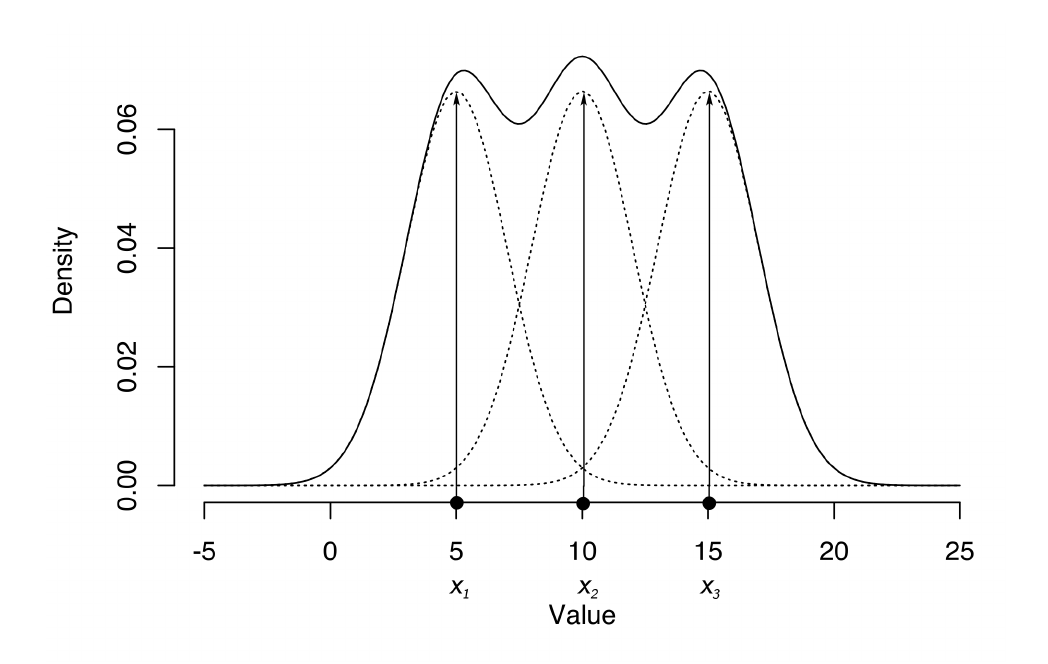
\includegraphics[scale=0.35]{dichte}
  \end{center}
  \vspace{-\baselineskip}
\end{figure}
Die Abbildung zeigt eine geglättete Dichtefunktion, auf jedem Datenpunkt $x_n$ liegt ein Gaußkern. Die Varianz $\sigma^2$ bestimmt die Stärke der Glättung, d.h. bei großer Varianz ist die Glättung stark und bei sehr kleiner ist die geglättete Dichtefunktion ähnlich der empirischen.

\subsubsection{What is the difference between GMM estimated with the EM algorithm and a kernel density estimation using the same samples with a Gaussian kernel?}

EM verwendet likelihood, diese ist parametrisiert. Gaußkern Methode ist nicht parametrisiert. GMM (Gaussian Mixture Model) ist einfach eine gewichtete Summe aus Gaussverteilungen.

\subsection{Explain the maximum likelihood method for estimation of probability density functions!}
\label{ML}
Gegeben sind die Daten $X = x_1, \cdots ,x_N$. Ziel ist es die Parameter $\Theta$ des parametrischen Modells zu schätzen (über Maximum Likelihood Schätzer). Bei der Maximum-Likelihood Methode werden die Parameter $\Theta$ so geschätzt, dass die Likelihood-Funktion maximal wird, dabei sind die Daten $X$ fixiert und die zu schätzenden Parameter $\Theta$ variieren.
Die Likelihood-Funktion ist definiert durch:
\begin{align*}
P(X|\Theta) = P(x_1, \cdots ,x_N | \Theta) = P(x_1|\Theta)P(x_2|x_1,\Theta) \cdots P(x_N|x_{N-1}, \cdots x_1,\Theta)
\end{align*}

\subsubsection{What happens if the samples are not i.i.d?}
\label{iid}Nur wenn sie independent and identically distributed sind, können wir die Likelihood-Funktion über das Produkt der Likelihoods aller $x_n$ bestimmen, d.h.
\begin{align*}
P(X|\Theta) = \prod_{n=1}^N P(x_n|\Theta)
\end{align*}

\subsection{Discuss statistical classification! How can the Bayes theorem be used in this context? Describe all variables and terms!}

Die Klassifikation von $N$ Samples $X=\{\langle x_1,t_1 \rangle, \cdots , \langle x_N,t_N \rangle\}$ bezüglich $c$ Klassen erfolgt anhand der Wahrscheinlichkeit $P(t|X)$ einer Objektbeschreibung $x$ zur Klasse $t$ zu gehören. Wenn man zum Beispiel mit einem 2-Klassenproblem zu tun hat, sieht man durch $P(t=1|x) > P(t=2|x)$ eindeutig die Zugehörigkeit. \\
\label{bayes}Diese posterior Wahrscheinlichkeit kann über den Satz von Bayes formuliert werden
\begin{align*}
\underbrace{P(t|x)}_{\text{posterior Wahrscheinlichkeit}} = \frac{\overbrace{P(x|t)}^{\text{Likelihood;}} \overbrace{P(t)}^{\text{prior Wahrscheinlichkeit}}}{\underbrace{P(x)}_{\text{Skalierungsfaktor}}}
\end{align*}
$P(x)$ skaliert $P(t|x)$ sodass $\sum_t P(t|x) = 1$ und der Skalierungsfaktor ist für alle Klassen $t$ gleich groß. Um die Klassenzugehörigkeit bestimmen zu können wählen wir jene Klasse mit der größten posterior Wahrscheinlichkeit. \\

\subsubsection{Discuss the following simplifications of the Bayes classifier and their implications on the classification results: Neglecting the denominator and usage of the logarithm.}

\subsubsection{Under which circumstances is the Bayes classifier equivalent to the maximum likelihood classifeir?}
When there is no biasing towards any class from prior knowledge. If we assume that the priors are equal and ignore them in the classification, the Bayes classifier is equal to the ML-classifier.

\subsection{Welche Verfahren zum Schätzen von Wahrscheinlichkeitsdichtefunktionen aus gegebenen Daten kennen sie? Beschreiben sie diese kurz!}

Maximum Likelihood (ML) Schätzer, siehe \ref{ML} \\
Bayes Schätzer, siehe \ref{bayes} (mit $\Theta$ statt $t$) \\
Im Unterschied zum ML-Schätzer, wo $\Theta$ deterministisch und unbekannt ist, wird beim Bayes Schätzer $\Theta$ als Zufallsvariable modelliert, d.h. für $\Theta$ existiert eine Wahrscheinlichkeitsdichtefunktion, die sogenannte a-priori Verteilung.

\subsubsection{Sie haben eine Liste von i.i.d Samples gegeben und wollen diese mit einer Gaußverteilung modellieren. Wählen sie eine der zuvor beschriebenen Schätzmethoden und beschreiben sie die Vorgehensweise.}

Siehe \ref{iid} \\
Im nächsten Schritt kann die Likelihood-Funktion logarithmiert werden, ist aber nicht zwingend notwendig. Durch das Logarithmieren kann anstatt des Produktes die Summe verwendet werden, damit werden numerische Probleme bei sehr großen $N$ vermieden. Die Log-likelihood Funktion ist:
\begin{align*}
L(X|\Theta) = \sum_{n=1}^N ln( P(x_n|\Theta))
\end{align*}

\subsection{Wozu dient der k-means Algorithmus?}

Ziel von k-means ist es, die Daten in k-Cluster zu teilen. Kann aus EM-Algo für GMMs hergeleitet werden.

\subsubsection{Welche Eigenschafter hat er (Initialisierung, Entscheidungsgrenze)?}
\begin{enumerate}
\item {\bf Initialisierung} Anzahl der Cluster und muss adäquat gewählt werden ebenso wie die Startpositionen der Schwerpunkte.
\item {\bf Entscheidungsgrenzen} werden gebildet über ein Voronoi-Diagram bezüglich der Schwerpunkte, geben Auskunft über die Zugerhörigkeit der Samples zu einem Cluster.
\end{enumerate}

\subsubsection{Welches Kriterium wird optimiert?}
Optimiert wird die Position der Cluster-Schwerpunkte bezüglich der minimalen kumulativen Distanz der einzelnen Samples zu den Schwerpunkten.

\subsection{Diskutieren sie Unterschiede und Gemeinsamkeiten von k-means und EM für Gaußsche Mischverteilungen (Einsatzgebiet, Datenmodelle, Konvergenzkriterium, Initialisierung, ...)}
EM kann Cluster unterschiedlicher Größe haben im Gegensatz zu k-means, kann korrelierte Cluster erkennen und repräsentieren durch die Kovarianzmatrix, kann mit unvollständigen Beobachtungen umgehen.
K-means versucht eine absolute Trennung der Daten während EM robuster ist bezüglich Punkten die in mehreren Clustern sein könnten. \\
{\bf Einsatzgebiet}: k-means zur Segmentierung in der Bildverarbeitung, wenn wir fixe Grenzen wollen. EM mehr in der Statistik. \\
{\bf Datenmodell}: Normalverteilungen \\
{\bf Konvergenz}: EM hat Zugehörigkeitswahrscheinlichkeiten die konvergieren, k-means nur die kumulative Distanz. \\
{\bf Initialisierung}: Bei k-means durch den Benutzer, welcher die Anzahl der Cluster angeben muss.

\subsection{Erklären sie, wie mittels PCA (Hauptkomponententransformation) und LDA (Linear Discriminant Analysis) Daten auf eine Dimension reduziert werden!}
Annahme: Varianz der Daten (Leistung) entspricht auch der Information. Wir versuchen also die Varianz der Daten zu maximieren. Bei der PCA wird die Kovarianzmatrix der gesamten Daten maximiert, während bei der LDA versucht wird, das Verhältnis zwischen Between-Class-Covariance und Within-Class-Covariance zu maximieren.

\subsubsection{Beides sind lineare Transformationen, wie wird jeweils der Transformationsvektor bestimmt?}
Bei PCA: Lösen durch Eigenvektoren der Kovarianzmatrix durch Lösen von $SU=UL$ \\
Bei LDA: Between-Class: $S_b = (m_{x,2}-m_{x,1})(m_{x,2}-m_{x,1})^T$, Within-Class: $u^TS_wu$

\subsubsection{Skizzieren sie ein Beispiel mit Daten aus dem ${\rm I\!R}^2$ und zeichnen sie die ungefähren Transformationsvektoren ein!}
\begin{figure}[htb]
  \begin{center}
  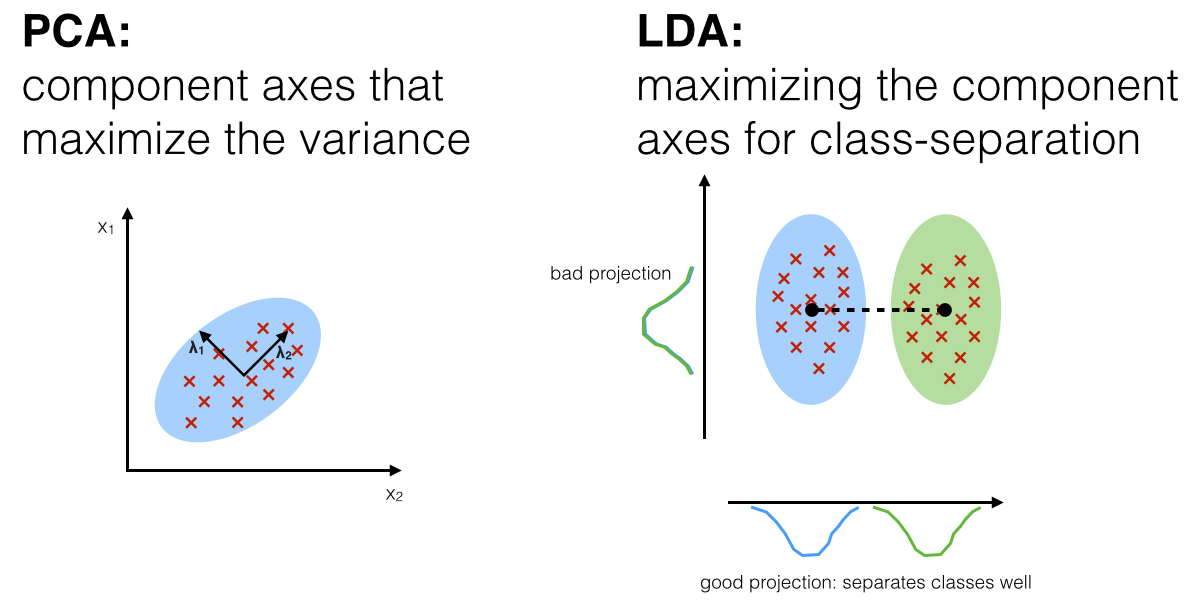
\includegraphics[scale=0.35]{pcalda}
  \end{center}
  \vspace{-\baselineskip}
\end{figure}

\subsection{Erklären sie ein Bayes'sches Netzwerk (d.h. ein gerichtetes graphisches Modell). Wie werden damit Wahrscheinlichkeiten modelliert?}

Knoten: Zufallsvariable \\
Kanten: Die bedingten Abhängigkeiten. Knoten die nicht miteinander verbunden sind sind voneinander Unabhängig \\
Jedem Knoten ist eine Wahrscheinlichkeitsfunktion zugeordnet. Jedem Knoten des Netzes ist eine bedingte Wahrscheinlichkeitsverteilung der durch ihn repräsentierten Zufallsvariable gegeben, die die Zufallsvariablen an den Elternknoten zuordnet.

\subsection{Sie haben mehrere HMMs mit Parametern $\Theta_k$ sowie eine Beobachtungssequenz $X = x_1, \cdots , x_N$. Wie kann man entscheiden, von welchem HMM die Beobachtungssequnz erzeugt wurde? Nennen sie eine Anwendung!}
Wir haben ein Evaluierungs-/Klassifizierungsproblem, daher benutzen wir den Forward/Backward Algorithmus. \\
Man berechnet also von jedem HMM mittles F/B-Algo die Wahrscheinlichkeit, dass $X$ von diesem HMM erzeugt wurde, und wählt das mit der größten Wahrscheinlichkeit. Anwendung: Spracherkennung (n-grams) \\

\subsubsection{Kann man den Viterbi-Algo hierzu benutzen?}
Siehe \ref{Viterbi}

\subsection{Beschreiben sie die statistische Klassifikation! Wie kann das Bayes Theorem dafür verwendet werden? Erklären sie die einzelnen Terme und Variablen!}
Siehe \ref{bayes}

\subsubsection{Welche statistische Information über die Daten unterscheidet den Bayes Klassifikator vom Maximum Likelihood (ML) Klassifikator?}
Die a-priori Anteilswahrscheinlchkeiten für das Auftreten einer Klasse sind bei Bayes bekannt aber bei ML unbekannt, daher wird eher ML bei Sprach-/Bildverarbeitung und Bayes bei Textverarbeitung verwendet.

\subsubsection{Gegeben sei ein 2-dimensionales 2-Klassen Problem. Unter welchen Modellannahmen bekommt man eine lineare Entscheidungsgrenze im Bayes Klassifikator?}
Bei gleichen und sphärischen Kovarianzmatritzen für alle Klassen.

\subsubsection{Bei der statistischen Klassifikation verwendet man oft die logarithmische Likelihood-Funktion. Kann die Verwendung des Logarithmus das Klassifikationsergebnis ändern (Begrüundung)?}
Das Klassifikationsergebnis bleibt das gleiche, da der Logarithmus eine monoton steigende Funktion ist und an der selben Stelle ein Maximum hat wie die ursprüngliche Funktion.

\subsection{Erklären sie den Unterscheid zwischen MM und HMM}
MM: Zustände können direkt von den Knoten abgelesen werden. \\
HMM: Die Zustände werden indirekt bestimmt, nur die Observer auf die Zustände emittieren bei Zustandswechsel den Zustand. Die Ereigniswahrscheinlichkeit wird in einer Matrix gespeichert und abgefragt.

\subsection{Erläutern sie die kernbasierte Schätzung von Wahrscheinlichkeitsverteilungen (insbesondere empirische und geglättete Dichtefunktionen)}
Kernbasierte Schätzungen gehören zu den nichtparametrischen Modellen. Diese versuchen mit möglichst wenigen Annahmen über die funktionale Form der Verteilung auszukommen und sind somit generisch einsetzbar. Der Preis dafür ist, dass das so gewonnene Modell sehr hohe Komplexität aufweist. \\
Die Empirische Dichtefunktion ist eine Summe von Dirak-Impulsen auf den Datenpunkten normiert durch die Anzahl der Datenpunkte. Sie hat maximale Auflösung, ist aber keine glatte Verteilungsfunktion. Um zu glätten wird in der Regel ein Gaußkern verwendet, dies liefert uns eine realitätsnährere Wahrscheinlichkeitsverteilung.

\subsection{Erklären sie den k-means Algorithmus!}
\begin{enumerate}
\item Initialisierung: Auswahl von k Cluster Zentren
\item Zuordnung: Jeder Datenvektor wird demjenigen Cluster zugeordnet, zu dessen Clusterzentrum die euklidsche Distanz minimal ist.
\item Die Clusterzentren werden in ihren jeweiligen neuen Mittelpunkt verschoben
\item Sollte sich die Zuordnung von Datenvektoren nicht mehr ändern dann fertig, sonst weiter mit $2)$
\end{enumerate}

\subsection{Wie bestimmt man die Transformationsmatrix der PCA?}
Über die Eigenvektoren der Kovarianz-Matrix durch Lösen von $SU=UL$

\subsection{Welche 3 Problemstellungen treten beim HMM auf? Erklären sie diese kurz (u.a. Algorithmus, Einsatzgebiet,...)}
\begin{enumerate}
\item Evaluierungs/Klassifikationsproblem \\
siehe \ref{eval} 
\item Dekodierungsproblem \\
Gegeben ist das Modell $\Theta$ und die Beobachtungssequenz $X=x_1, \cdots x_N$. Gesucht ist $Q^*=\text{arg }max_Q[P(Q|X,\Theta)]$. $Q^*$ bezeichnet eine Zustandsfolge (=Statesequenz) die eine Beobachtungssequenz $X$ bei gegebenen Paramtern $\Theta$ am besten erklärt. Der Viterbi Algorithumus wird zur Ermittlung von $Q^*$ verwendet.
\item Schätzproblem (Lernproblem) \\
Gegeben sind $R$ Beobachtungssequenzen $X^{1:R}=X^1, \cdots ,X^R$, gesucht sind die Parameter $\Theta$ des Modells, d.h.
\begin{align*}
\Theta_{ML}=\text{arg }\underset{\Theta}{max}[P(X^{1:R}|\Theta)] = \text{arg }max[\prod_{r=1}^R P(X^r|\Theta)]
\end{align*}
wobei $P(X^r|\Theta)$ die Likelihood des Evaluierungsproblems darstellt. Die ML Lösung $\Theta_{ML}$ kann mit dem EM-Algorithmus gefunden werden.
\end{enumerate}

\subsection{Erklären sie kurz ein Markov Netzwerk (d.h. ein ungerichtetes graphisches Modell). Wie werden damit Wahrscheinlichkeitsverteilungen modelliert?}
Markov networks, also known as Markov random fields (MRFs) are represented by undirected graphs. As in Bayes Networks, MNs encode certain factorization and conditional independence properties of the joint probability distribution. \\
A Markov Network is a tupel $M = (G,\{\Psi_{C_1}, \cdots ,\Psi_{C_L}\})$ where $G=(X,E)$ is an undirected graph with maximal cliques $C_1, \cdots C_L$. The nodes $X$ correspond to nonnegative functions called factors or potentials, and define a probability distribution in combination with a normalization constant $Z$.

%%%%%%%%%%%%%%%%%%%%%%%%%%%%%%%%%%%%%%%%%%%%%%%%%%%%%%%%%%%%%%%%%%%%%%%%%%%%%%%%%%%%%%%%%%%%

\newpage
\pagestyle{index-style}
\tableofcontents{}

\end{document}
